\documentclass[11pt, oneside]{article}   	% use "amsart" instead of "article" for AMSLaTeX format
\usepackage{geometry}                		% See geometry.pdf to learn the layout options. There are lots.
\geometry{letterpaper}                   		% ... or a4paper or a5paper or ... 
%\geometry{landscape}                		% Activate for for rotated page geometry
%\usepackage[parfill]{parskip}    		% Activate to begin paragraphs with an empty line rather than an indent
\usepackage{graphicx}				% Use pdf, png, jpg, or eps� with pdflatex; use eps in DVI mode
								% TeX will automatically convert eps --> pdf in pdflatex		
\usepackage{amssymb}
\usepackage{amsmath}
\usepackage{parskip}
\usepackage{color}
\usepackage{hyperref}

\title{Integrating zz + 1}
%\author{The Author}
%\section{}
%\subsection*{}
\date{}							% Activate to display a given date or no date

\graphicspath{{/Users/telliott_admin/Dropbox/Tex/png/}}
% \begin{center} 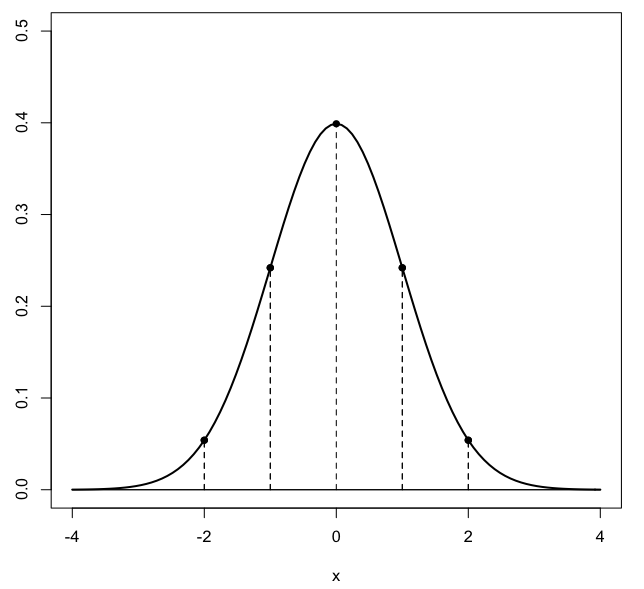
\includegraphics [scale=0.4] {gauss3.png} \end{center}
\begin{document}
\maketitle
\Large
This problem is Beck 4.26.  Consider 
\[ f(z) = \frac{1}{z^2 + 1} \]
We see that the denominator is zero when
\[ z^2 = -1, \ \ \ z = \pm \ i \]
Suppose our curve is the unit circle centered at $i$, designated as $C[i,1]$.  Obviously, this curve contains the singularity $z = i$.  Now
\[ z^2 + 1 = (z + i) (z-i) \]
Rewrite the function as
\[ f(z) = \frac{1/z+i}{z-i} \]
Then
\[ \int \frac{1}{z^2 + 1} \ dz = \int \frac{1/z+i}{z-i} \ dz \]
Cauchy's Integral formula says that
\[ f(w) = \frac{1}{2 \pi i} \ \oint  \frac{f(z)}{z-w} \ dz \]
The value of the function is
\[ \frac{1}{z+i}(i) = \frac{1}{2i} \]
and the integral in question is then.
\[ 2 \pi i f(w) = \pi  \]
\[ \int \frac{1}{z^2 + 1} \ dz = \pi \]

Similarly, if the unit circle is centered at $-i$, rewrite the function as
\[ f(z) = \frac{1/z-i}{z+i} \]
The value of the function is
\[ \frac{1}{z-i}(-i) = -\frac{1}{2i} \]
and that integral is then $- \pi$.

A contour that includes both singularities integrates to zero.

\subsection*{connection reals}
Note that for the real function
\[ \int_0^{\infty} \frac{1}{1 + x^2} \ dx \]
We know the answer to this one, it is 
\[ \tan^{-1} x \ \bigg |_0^{\infty} = \frac{\pi}{2}  \]
Since $f(x)$ is an even function, the integral over $-\infty \rightarrow \infty = \pi$, and we feel there ought to be some connection between the two real and complex results.

Suppose we draw a part of the contour from $-\infty \rightarrow \infty$ on the real axis.  That integral is $\int f(z) \ dz$ but $y$ and $dy$ are both zero so it is just $\int f(x) \ dx$ with the result which we just obtained.

How to complete the contour?  Imagine the hemisphere in the upper half-plane with $R$ at $\infty$.  That is, parametrize
\[ \gamma(\theta) = Re^{i\theta}, \ \ \ \theta \in [0, \pi] \]
\[ \gamma \ '(\theta) =  iRe^{i\theta} \]
The integral is
\[ \int_0^{\pi} \frac{1}{1 + R^2 e^{i2\theta}} \ i R e^{i \theta} \ d \theta \]
Now what?
the 
It's clear that as $R \rightarrow \infty$, this integrand goes to 0.


\end{document}  